%%% -*- TeX-master: "../main" -*-
\chapter{From Time Series to Label Sequences}
\label{cha:methods}

\begin{figure}[h]
  % Center this figure specifically because it is wider than \textwidth
  \makebox[\textwidth][c]{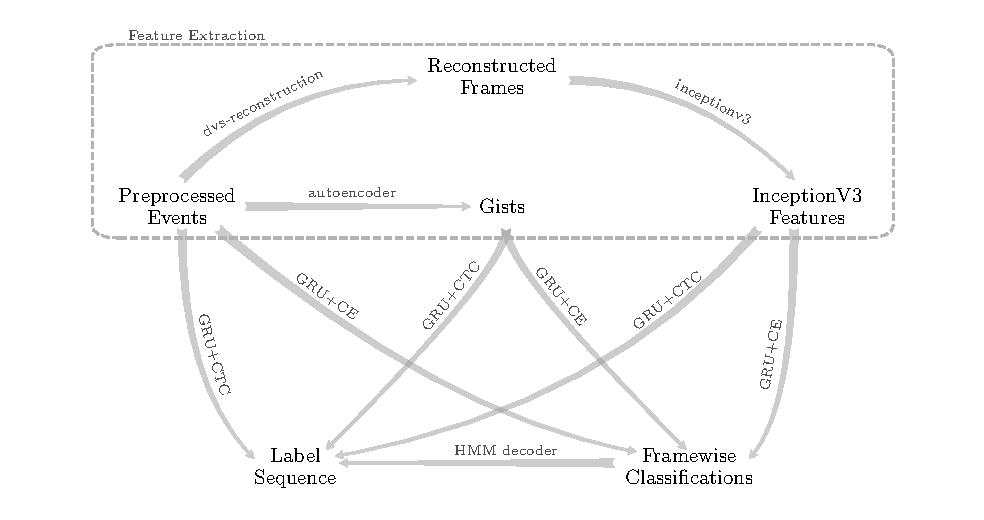
\includegraphics{figures/methods/overview}}
  \caption{Overview of the methods and intermediate representations used in this
    thesis}
  \label{fig:method-overview}
\end{figure}

There are three types of sequence labeling tasks defined by Graves. The first is
sequence classification where the data is a set of sequences each of which
belongs to a single class. This problem can be generalized to segment
classification. Here a data point is subdivided into one or more segments with
known start and end points and each of them needs to be classified. Splitting
the inputs along the segment boundaries and interpreting the problem as a
sequence classification task is not equivalent because the segment classifier
may and often will use surrounding context to disambiguate ambiguous segments.
The most general task is called temporal classification in which neither the
number of classes per sequence nor any segment boundaries are known. The only
assumption is that an input has at most as many labels as the length of the
input sequence. Such a classifier has to compute just the label sequence, though
some of them can optionally also return a segmentation.

The problem of gesture recognition from address-event data falls into the last
category. A recording may contain any number of gestures at arbitrary points in
time and each gesture takes up a varying number of events depending on distance
between hand and DVS, speed of execution and lighting conditions. Figure
\ref{fig:method-overview} depicts all the ways that we tried to solve this
temporal classification task. All of them include recurrent neural networks
(RNNs) because they are the state of the art in sequence learning. There are two
popular ways to compute a label sequence from an input. The older one combines
an RNN and a hidden Markov model (HMM). The RNN provides localized
classifications of each sequence element and the HMM segments the input on the
basis of the RNN output and deduces the most likely label sequence. These are
all paths in Figure \ref{fig:method-overview} that leave the feature extraction
phase and take \emph{framewise classifications} as an intermediate step to
\emph{label sequence}. \citeauthor{ctc} devised a method called connectionist
temporal classification (CTC) that combines both steps, RNN classification and
HMM decoding, by means of a new loss function for neural network training. This
enables a neural network in theory to solve any temporal classification task
end-to-end. This approach is represented in Figure \ref{fig:method-overview} by
all paths labeled \texttt{GRU+CTC} that lead to \emph{label sequence} directly.

Neural networks that are capable of sequence-to-sequence transformations rely on
circular connections in their computational graph and are called recurrent
neural networks. They process an input sequence element by element and the
recurrent connections allow them to carry information, and thus context, from
step to step. The particular variant of RNN we use is called a gated recurrent
unit, GRU for short, which allows the networks to learn much longer temporal
relationships than a naive RNN could. We introduce RNNs, GRUs and their
predecessor, the long short-term memory layer, in Section \ref{sec:rnns}.

In the beginning, we applied both methods to the 25-gesture dataset, however CTC
training did not produce any result at all and framewise classification levelled
off at about 40\% accuracy, which we deemed to low for successful decoding. The
type of data that we are handling consists of very long sequences with only
minimal information content per sequence element and a high noise ratio. The
recordings average 30,000 events per second and single gestures often span over
100,000 events. Even though we employ gated recurrent units that can learn
relationships over hundreds of timesteps, we assumed that the network might be
just overwhelmed by the data. Moreover, we conjectured that the continuous time
and consequential variance in event density over time made the task more
difficult. We introduced two feature extraction methods with the specific goal
of overcoming these problems. Both compress sequences of varying length into
fixed-length vectors. That lets us transform the continuous-time sequences into
discrete-time ones by grouping the events into time windows of fixed length but
varying numbers of events and compress them into fixed-length vectors. The
transformed sequences should improve learning because the number of data points
per second is cut down and the data points are enriched with the information of
all events then went into them. On the original data, the network had to rely
almost purely on the context, because a single event is uninformative.
Afterwards, each data point should be quite meaningful on its own.

% TODO: Train CNN classifier on gists to check how much context is actually
% necessary

The first method reconstructs grayscale images from the event data (Section
\ref{sec:frame-reconstruction}) and then uses a pre-trained image classification
network to extract visual features (Section \ref{sec:inceptionv3}). The second
idea, explained in Section \ref{sec:autoencoder}, uses a specific type of
network, an autoencoder, to learn an efficient compression directly. We call the
representations learned by the autoencoder \emph{gists} because they encode the
gist of the input.

Section \ref{sec:framewise} explains framewise classification and the network
architecture that we use for that task and all that follow. These local
classifications are decoded with an HMM which is described in Section
\ref{sec:hmm}. In Section \ref{sec:hmm-segmentation} we split the decoding
process into two phases, first the input is segmented which is followed up by
segment classification, both with an HMM. Lastly, we introduce connectionist
temporal classification in Section \ref{sec:ctc} and explain how it combines the
steps of classification and decoding into one.

\section{Recurrent Neural Networks}
\label{sec:rnns}

The classical neural network is a parametric function approximator that takes an
input vector of fixed length and produces an output vector of fixed length.
Recurrent neural networks generalize either input, output or both to sequences.
Let $x^{(n)}$ be a sequence of input vectors and define a simple network with
one hidden layer. So it has a weight matrices $W$, $V$, a bias $b$ and in this
example we will use a $\tanh$ non-linearity. The naive way to produce an output
sequence $y^{(n)}$ would be to apply the network elementwise by
\begin{align*}
  h^{(t)} & = \tanh\left( Wx^{(t)} + b \right)\\
  y^{(t)} & = Vh^{(t)}
\end{align*}
where $h^{(t)}$ are the activations in the hidden layer for the $t$-th sequence
element. However, this network does not have access to any historical context
and so it will have a difficult time to, for example, recognize gestures which
are inherently temporal. One solution is to introduce recurrent connections
between layers in the form of an additional dependency of $h^{(t)}$ on $h^{(t -
  1)}$. In precise terms this means that we add another weight matrix $U$ to the
network and redefine it as
\begin{align*}
  h^{(t)} & = \tanh\left( Wx^{(t)} + Uh^{(t - 1)} + b \right)\\
  y^{(t)} & = Vh^{(t)}
\end{align*}
where $h^{(0)}$ is initialized arbitrarily, though with the zero vector most of
the time. This network now has memory, so to speak, in the form of $h^{(t)}$
that allows it to take the history of the sequence into account.

Though fine in theory, in practice this type of RNN suffers from the vanishing
gradient problem. When such a network is trained with some form of gradient
descent, the gradient decays exponentially quickly as it propagates back through
time. This makes it hard for such a network to solve tasks that require more
than about 10 steps of temporal contrast. \citeauthor{lstm} solved this with the
introduction of long short-therm memory (LSTM) layers that they designed to
allow constant error flow \cite{lstm}. Instead of carrying over the state of the
hidden layer directly, the LSTM architecture replaces the hidden layer with a
subnetwork that explicitly controls which memories should be forgotten and which
should be overwritten. This keeps the gradient magnitude large and provides
sufficient signal for learning over several hundred timesteps. An LSTM layer
consists of two persistent states, the cell state $c^{(t)}$ and the hidden state
$h^{(t)}$, and three gates, the input, output and forget gates $i^{(t)}$,
$o^{(t)}$ and $f^{(t)}$, respectively, which control the flow of information.
They are connected as follows where $\sigma$ is the logistic sigmoid function
and $\circ$ denotes an element-wise product.
% TODO: Explain the logistic sigmoid?
\begin{align*}
  f^{(t)} & = \sigma\left( W_{f}x^{(t)} + U_{f}h^{(t - 1)} + b_{f} \right)\\
  i^{(t)} & = \sigma\left( W_{i}x^{(t)} + U_{i}h^{(t - 1)} + b_{i} \right)\\
  o^{(t)} & = \sigma\left( W_{o}x^{(t)} + U_{o}h^{(t - 1)} + b_{o} \right)\\
  c^{(t)} & = f^{(t)} \circ c^{(t - 1)} + i^{(t)} \circ \tanh\left( W_{c}x^{(t)} + U_{c}h^{(t - 1)} + b_{c} \right)\\
  h^{(t)} & = o^{(t)} \circ \tanh\left( c^{(t)} \right)
\end{align*}
The forget and input gates control the updates to the cell state while the
output gate controls which parts of the cell state are written out into the
hidden state and thus into the output of the layer. A later version called
Peephole LSTM uses the cell state directly instead of the previous hidden state
to compute the input, output and forget gates.

% TODO: tikz pictures of RNN, LSTM and GRU computational graphs

In \citeyear{gru} \citeauthor{gru} published a simplification of LSTM called a
gated recurrent unit (GRU) \cite{gru}. They merge the cell state into the hidden
state $h^{(t)}$, combine the input and forget gates into a single update gate
$z^{(t)}$ and replace the output gate with a reset gate $r^{(t)}$ that has no
equivalent in LSTM. A GRU layer is then defined by
% TODO: Mention z and (1 - z)
\begin{align*}
  r^{(t)} & = \sigma\left( W_{r}x^{(t)} + U_{r}h^{(t - 1)} \right)\\
  z^{(t)} & = \sigma\left( W_{z}x^{(t)} + U_{z}h^{(t - 1)} \right)\\
  h^{(t)} & = z^{(t)} \circ h^{(t - 1)} + \left( 1 - z^{(t)} \right) \circ \tilde{h}^{(t)}\\
  \tilde{h}^{(t)} & = \tanh\left( Wx^{(t)} + U\left( r^{(t)} \circ h^{(t - 1)} \right) \right).
\end{align*}
where $\tilde{h}^{(t)}$ is an intermediate variable. This architecture has fewer
parameters and operations then LSTM which makes it easier to implement and
compute which reduces training time. \citeauthor{gruvslstm} have found that GRU
performance is comparable to LSTM \cite{gruvslstm}. For these reasons, we have
decided to rely on GRUs in this thesis.

\section{Frame Reconstruction}
\label{sec:frame-reconstruction}

The DVS only reacts to changes in light intensity. This removes all the
redundant information about stationary objects that makes up the bulk of the
data in videos consisting of consecutive frames. Furthermore, the remaining
information about the illumination gradient at a point is coarsely discretized
and carries just a single bit of information, the sign of the change.
Nonetheless, two groups have shown that it is still possible to reconstruct
grayscale images from the data \cite{bardow2016,reinbacher2016}.
\citeauthor{reinbacher2016} interpret the events as points on an event manifold
which they reconstruct by minizing an energy including a smoothness regularizer
over it with variational methods. The solution can then be interpreted as an
intensity image.

They have published an open-source implementation of their algorithm which we
used to reconstruct images from the dataset. We created one image every
\SI{2.5}{\milli\second} resulting in 400 frames per second. Figure
\ref{fig:reconstructed} showcases three frames depicting a \texttt{swipe-down}
gesture. For one thing, the subject's hand has been resolved reasonable well and
it has been reconstructed as one smooth surfaces with shadows creating an
illusion of depth and even individual digits are visible. At the same time
though, artifacts are accumulating in the background regions of the image and
over time the images become darker. The reason for this is most likely that we
mounted the camera on a stand. As a result it was static relative to the
background which therefore produced no events.

\begin{figure}[h]
  \centering
  \begin{subfigure}{\textwidth}
    \hspace*{\fill}
    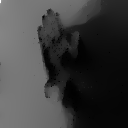
\includegraphics[width=0.3\textwidth]{figures/methods/reconstructed-1}
    \hspace*{\fill}
    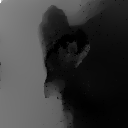
\includegraphics[width=0.3\textwidth]{figures/methods/reconstructed-2}
    \hspace*{\fill}
    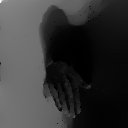
\includegraphics[width=0.3\textwidth]{figures/methods/reconstructed-3}
    \hspace*{\fill}
  \end{subfigure}
  \caption{Reconstructed frames showing a \texttt{swipe-down} gesture}
  \label{fig:reconstructed}
\end{figure}

\section{Feature Extraction with an InceptionV3 Network}
\label{sec:inceptionv3}

It is an emergent property of neural networks trained on image tasks that they
develop increasingly abstract features in higher levels of the network. So the
bottom layers of a network will learn to recognize simple shapes like edges in
various orientations or corners. On top of these, the network learns to
recognize more complex shapes like circles or rectangles. This continues through
the network and in the highest layers you find neurons that recognize faces or
cars. An insight from transfer learning says that these learned features can be
reused across a variety of tasks because only a handful of layers at the top
will be completely task specific. So by reusing a pre-trained network and
replacing the top layers you can reach high performance on a new task in a
fraction of the time it would take to train the whole network from scratch. In
our case, reusing a network pre-trained on a large dataset has the additional
advantage that we can indirectly make use of a lot more training data than what
our dataset provides.

\begin{figure}[h]
  \centering
  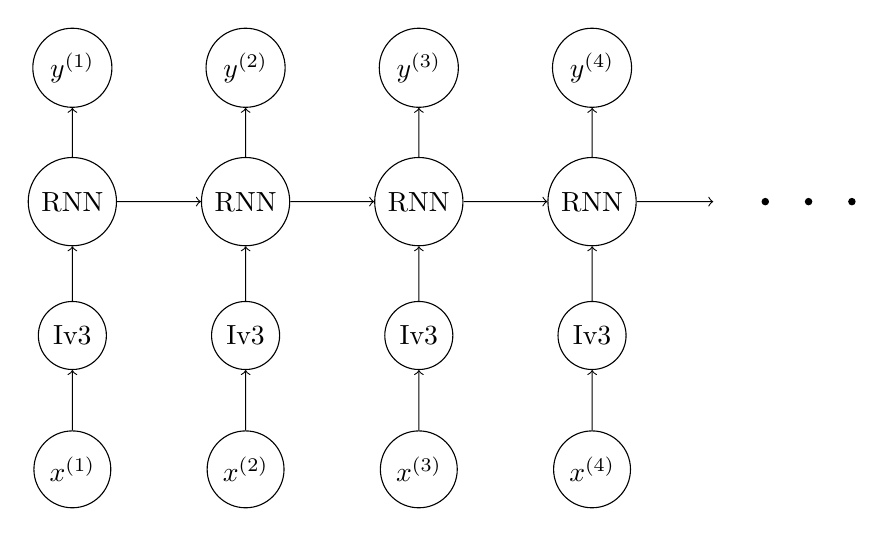
\begin{tikzpicture}[xscale=2.2,yscale=1.7]
    \foreach \t in {1, 2, 3, 4} {
      \node[draw,circle](x\t) at (\t, 0) {$x^{(\t)}$};
      \node[draw,circle](i\t) at (\t, 1) {Iv3};
      \node[draw,circle](r\t) at (\t, 2) {RNN};
      \node[draw,circle](y\t) at (\t, 3) {$y^{(\t)}$};

      \draw[->] (x\t) -- (i\t);
      \draw[->] (i\t) -- (r\t);
      \draw[->] (r\t) -- (y\t);
    }

    \foreach \t [evaluate=\t as \tnext using int(\t + 1)] in {1, 2, 3} {
      \draw[->] (r\t) -- (r\tnext);
    }

    \draw[->] (r4) -- (4.7,2);
    \foreach \p [evaluate=\p as \x using (5 + 1/4 * \p)] in {0, 1, 2} {
      \fill (\x, 2) node[draw,circle,fill,inner sep=0,minimum size=0.08cm]{};
    }
  \end{tikzpicture}
  \caption{Computational graph of an RNN on top of an InceptionV3 network}
  \label{fig:iv3-rnn}
\end{figure}

The end goal is to compress sequences of events into more expressive data
points. The idea for that is that we reconstruct grayscale images from the event
data and then feed these to a pre-trained network that is able to extract
abstract and meaningful features about the subjects hand position from them. In
particular, we chose an InceptionV3 network \cite{inceptionv3} implemented in
keras \cite{chollet2015keras} that was pretrained on the ImageNet dataset to
5.6\% top-5 accuracy. We cut off the fully connected layers that are specialized
on ImageNet and stored the output of the hidden layer at that depth as feature
vectors to later train an RNN on. This setup is basically equivalent to the
network whose computational graph is sketched in Figure \ref{fig:iv3-rnn}. There
an InceptionV3 network is run on each sequence element with an RNN running on
top for temporal context. The difference to the depicted network is that we
precompute all the intermediate outputs. The advantage is that the deep network
need not be rerun on each epoch. However, its weights are also practically
frozen, so they will not be fine-tuned to our problem. One detail worth noting
is that the InceptionV3 network expects RGB images with a resolution of
299$\times$299 pixels. To make the 128$\times$128 pixel grayscale images
compatible with these requirements we scaled them up and duplicated each of them
three times into the three color channels of an RGB image.

\section{Representation Learning with an Autoencoder}
\label{sec:autoencoder}

An autoencoder is a neural network that takes an input and reproduces it, so it
is approximating the identity function. There are different flavors to this
concept, though we are going to focus on the type that is in some form
hour-glass shaped. That means that at some intermediate point in the network the
data has to flow through a funnel, a layer whose output dimensionality is
smaller than the network input. This forces the network to learn a
low-dimensional representation of the input data from which it can later
reconstruct the input. The advantage of using a neural network for
dimensionality reduction is that the mapping can be highly non-linear and it
works on sequences.

\begin{figure}
  \centering
  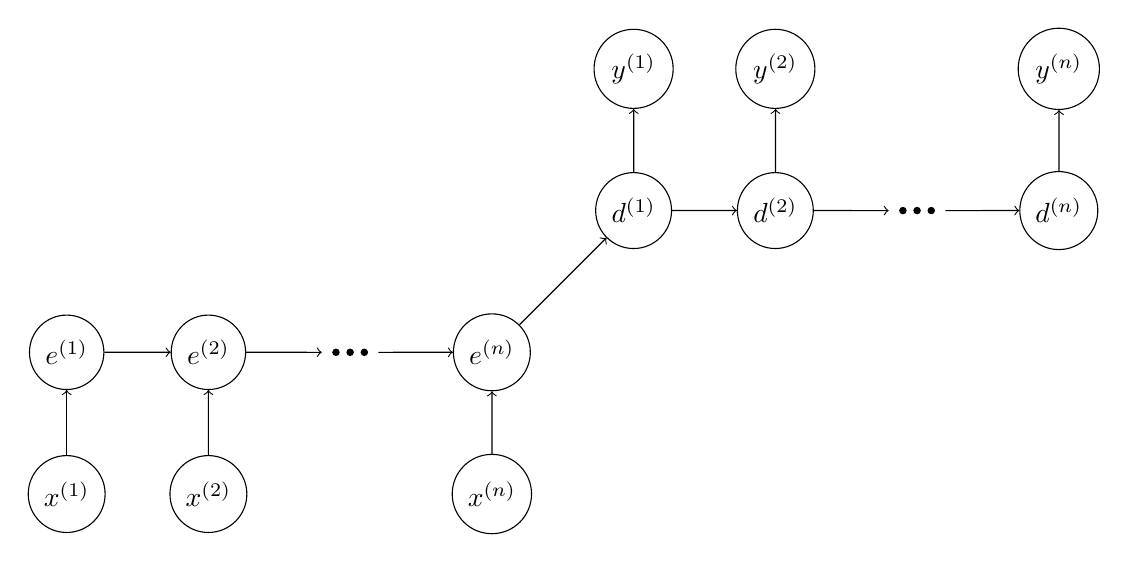
\begin{tikzpicture}[scale=1.8]
    \node[draw,circle](x1) at (0, 0) {$x^{(1)}$};
    \node[draw,circle](x2) at (1, 0) {$x^{(2)}$};
    \node[draw,circle](xn) at (3, 0) {$x^{(n)}$};
    \node[draw,circle](e1) at (0, 1) {$e^{(1)}$};
    \node[draw,circle](e2) at (1, 1) {$e^{(2)}$};
    \node[draw,circle](en) at (3, 1) {$e^{(n)}$};

    \fill (1.9, 1) node[draw,circle,fill,inner sep=0,minimum size=0.08cm]{};
    \fill (2.0, 1) node[draw,circle,fill,inner sep=0,minimum size=0.08cm]{};
    \fill (2.1, 1) node[draw,circle,fill,inner sep=0,minimum size=0.08cm]{};
    
    \draw[->] (x1) -- (e1);
    \draw[->] (x2) -- (e2);
    \draw[->] (xn) -- (en);

    \draw[->] (e1) -- (e2);
    \draw[->] (e2) -- (1.8, 1);
    \draw[->] (2.2, 1) -- (en);

    \node[draw,circle](y1) at (4, 3) {$y^{(1)}$};
    \node[draw,circle](y2) at (5, 3) {$y^{(2)}$};
    \node[draw,circle](yn) at (7, 3) {$y^{(n)}$};
    \node[draw,circle](d1) at (4, 2) {$d^{(1)}$};
    \node[draw,circle](d2) at (5, 2) {$d^{(2)}$};
    \node[draw,circle](dn) at (7, 2) {$d^{(n)}$};
    
    \fill (5.9, 2) node[draw,circle,fill,inner sep=0,minimum size=0.08cm]{};
    \fill (6.0, 2) node[draw,circle,fill,inner sep=0,minimum size=0.08cm]{};
    \fill (6.1, 2) node[draw,circle,fill,inner sep=0,minimum size=0.08cm]{};
    
    \draw[->] (d1) -- (y1);
    \draw[->] (d2) -- (y2);
    \draw[->] (dn) -- (yn);

    \draw[->] (d1) -- (d2);
    \draw[->] (d2) -- (5.8, 2);
    \draw[->] (6.2, 2) -- (dn);

    \draw[->] (en) -- (d1);
  \end{tikzpicture}
  \caption{Sketch of our autoencoder architecture that encodes an input sequence
    $x$ of length $n$ into hidden states $e$. The decider is trained to decode
    the last hidden state $e^{(n)}$ into a sequence $y^{(1)}, \dots, y^{(n)}$
    resembling the input.}
  \label{fig:autoencoder-architecture}
\end{figure}

Our autoencoder follows the architecture proposed in \cite{gru}, alongside GRU,
for neural machine translation. See Figure \ref{fig:autoencoder-architecture}
for a sketch. The idea is that the network is split into an encoder and a
decoder which share information only along a single edge in the computational
graph. This edge initializes the decoder's hidden state with the final hidden
state of the encoder. It is the figurative funnel in the network because it has
to encode the complete input sequence. For that reason we call these encodings
the \emph{gist} of the input.

The specifics of the architecture are influenced by our requirements. We want to
use the encoder part to transform variable length event sequences of fixed
duration into fixed-length vectors. So the network architecture needs to
accomodate inputs of variable length and accordingly also be variable regarding
the output length. The preprocessed events are vectors in $\mathbb{R}^{5} \times
\{ -1, 1 \}$, so the features are partly continuous. It is common practice to
train an autoencoder to produce a probability distribution over sequences
instead of sequences directly. The original architecture is designed to work
over a finite alphabet and produces parameters for a multinoulli distribution
over that alphabet. So each $y^{(i)}$ is a non-negative vector whose entries sum
up to 1 and its $j$-th entry encodes the networks belief that the $j$-th word
should be placed at this point in the output sequence.

The continuity of the features requires a distribution over the real numbers.
\citeauthor{handwriting} uses an LSTM-RNN to generate handwriting where each
sequence element is a vector in $\mathbb{R}^{2} \times \{ 0, 1 \}$ encoding the
pen's $x$ and $y$ coordinates and whether it is currently lifted from the
blackboard \cite{handwriting}. Their network's output parameterizes a
distribution that is a mixture of Gaussians over the real attribute and a
Bernoulli distribution over the categorical attribute. They call such networks
\emph{mixture density networks}.

Our network handles an input sequence of length $n$, where $n$ is variable, by
encoding the complete sequence first. The it applies the decoder to produce a
distribution over a sequence of length $n$ and computing a loss between the two
sequences for training. We chose to produce an output sequence of the correct
length directly instead of learning a special \texttt{end-sequence} output
because our inputs are just arbitrary slices of events as opposed to sentences
in machine translation that have a meaningful end.

The architecture for our mixture density autoencoder is as follows. Both the
encoder and decoder are 3 layers of GRUs each of which has 256 units. Encoder
and decoder structure are necessarily symmetrical since the decoder is fed the
hidden state from the encoder. The encoder receives preprocessed events in
$\mathbb{R}^{6}$. Remember that the polarity has been standardized as well, so
it is not necessarily restricted to $\{ -1, 1 \}$ anymore. However, for purposes
of computing the loss, we rediscretize it again by mapping positive values to
$1$ and vice versa. The decoder produces parameters for a 10 component mixture
distribution of Gaussians with diagonal covariance matrices over
$\mathbb{R}^{5}$ and a single parameter for a Bernoulli distribution over $\{
-1, 1 \}$. This adds up to 10 component weights, $10 \cdot 5 = 50$ mean
parameters, $10 \cdot 5 = 50$ diagonal convariance matrix entries and a single
Bernoulli parameter, so 111 parameters in total. To project its 256-dimensional
output into the $\mathbb{R}^{111}$, the decoder has a single fully-connected
layer with weight matrix and bias term but without non-linearity on top.

The loss is the negative log-likelihood of the input sequence according to the
output distribution. To compute this, the outputs, which are arbitrary vectors in
$\mathbb{R}^{111}$, need to satisfy certain conditions. Therefore, except for the
Gaussian mean vectors $\mu$, all of them are transformed non-linearly. The
component weights $w_{i}$ are transformed with a softmax operation
\begin{equation*}
  w_{i} := \frac{\exp(w_{i})}{\sum_{j} \exp(w_{j})}
\end{equation*}
that ensures that the weights are between $0$ and $1$ and sum up to $1$. The
variance terms $\sigma_{ij}$ have to be positive so that the covariance matrix
is positive-definite. This is achieved with the softmax operation
\begin{equation*}
  \sigma_{ij} := \log\left( 1 + \exp(\sigma_{ij}) \right)
\end{equation*}
which ensures that a value is positive and is basically $\max\{ 0, \sigma_{ij}
\}$ with a rounded corner at $0$ which also never quite gets to $0$ as
$\sigma_{ij} \rightarrow -\infty$. Finally, the Bernoulli parameter $p$ is
squashed into the $(0, 1)$ range by the logistic sigmoid function
\begin{equation*}
  p := \sigma(p) = \frac{1}{1 + e^{-p}}.
\end{equation*}

The training setup is the same as for all networks trained for this thesis. We
use minibatch gradient descent with batches of size 32. The optimizer is Adam,
an optimization method that adaptively scales the learning rate for each
parameter \cite{adam}. Though it might be unnecessary with Adam, we still
employed exponential learning rate decay with $0.95$ to the power of the current
epoch. Lastly, we clip the gradients at a norm of $5$ which Graves recommends.
This also helps with numerical instabilities in case the covariances of the
mixture distribution should become really small.

Training recurrent neural networks on long sequences requires lots of memory
because all intermediate results over all timesteps need to be stored for
back-propagation. To avoid running out of memory, we split input sequences above
a maximum length into chunks. A chunk is similar to a batch, though the hidden
states are not cleared in between and they are trained on in order. So a batch
of sequences of length 100 might be split into five chunks where the first chunk
would contain the first twenty elements of all sequences and so forth. In
theory, this restricts the maximum distance in time over which the network can
learn relationships to the chunk size. In practice, we did not notice anything
that we would have traced back to this effect.

The autoencoder was trained on chunks of length 250, while all other networks
were trained with chunks of length 1000. The reasons for that are twofold.
First, the autoencoder is actually two recurrent networks in sequence, so a
chunk size of 250 means the memory requirements of a chunk size of 500. Second,
the autoencoder includes more expensive operations and was trained on a lot of
data. Because of this, training an autoencoder takes several days, while the
other networks can be trained in a matter of hours. Furthermore, the input data
of the autoencoder is special. In contrast to all classifier networks, the
autoencoder runs on variable length sequences. A batch of
\SI{2.5}{\milli\second} time windows of events has a long-tail distribution of
lengths. While most sequences will be quite short, one or two will be
significantly longer. The library we use requires us to effectively zero-pad all
sequences to the same length, which incurs large and unnecessary memory and
computational costs. Chunking allows us to cut down on these by excluding
sequences that have already ended in later chunk iterations.

\begin{figure}[h]
  \centering
  \begin{subfigure}{0.49\textwidth}
    \centering
    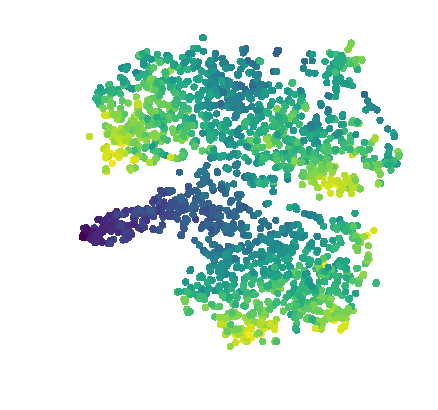
\includegraphics{figures/methods/tsne/thumbs-up}
    \caption{Thumbs up}
  \end{subfigure}
  \begin{subfigure}{0.49\textwidth}
    \centering
    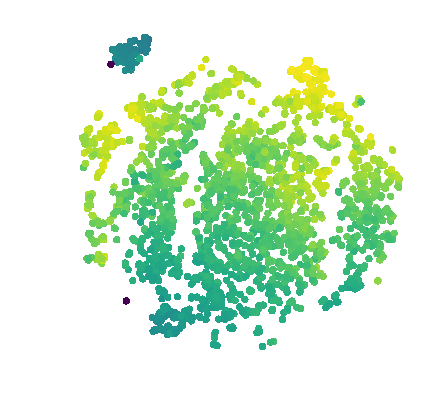
\includegraphics{figures/methods/tsne/swipe-left}
    \caption{Swipe left}
  \end{subfigure}
  \caption{t-SNE plots of learned representations of \SI{2.5}{\milli\second} segments}
  \label{fig:autoencoder}
\end{figure}

A last detail about the autoencoder structure is that the decoder is fed the
desired output of the previous timestep as input for the current timestep. Using
the terminology of Figure \ref{fig:autoencoder-architecture}, $d^{(2)}$ would be
fed $x^{(1)}$ as input. This is supposed to improve decoding performance because
the network can more easily keep track of its current position in the sequence. 

An interesting question is if the autoencoder has a denoising effect on the
representation. The noise is more or less uniformly distributed over the field
of view. Thus, the expected value of the loss incurred by noise should be $0$ in
expectation and the effect through gradient descent on the network should cancel
out in the long run. Therefore one might assume that the learned representation
is less noisy than its input.

% TODO: Maybe explain t-SNE

Figure \ref{fig:autoencoder} shows two t-SNE plots of learned representations.
Each point represents \SI{2.5}{\milli\second} of events and they are colored by
the number of events that went in them where a brighter color denotes more
events. Note that the axes carry no meaning in a t-SNE plot and all information
is in the distance between points. The key observation is that the points form
some high-dimensional structure that encodes, among others, the event density in
a segment.

\section{Framewise Classification}
\label{sec:framewise}

Methods with an explicit decoding step require localized classifications that
can be decoded into global classifications. In accord with Graves, we call this
\emph{framewise classifications}. Once again we use an RNN for that. This time
we are back in the domain of finite alphabets since the network should assign
each frame to one of 17 classes, 16 gestures plus the \texttt{<blank>} label.

To make our approaches comparable, we will use the same network architecture
throughout the rest of the thesis. It consists of three GRU layers with 256
units each, two fully-connected layers with $\tanh$ activations and also 256
units each and finally a fully-connected layer without activation function that
projects the output down into $\mathbb{R}^{17}$. The output is transformed with
softmax to parameterize a multinoulli distribution over the output classes which
encodes the networks belief that the current frame belongs to a certain class.

The loss function to optimize is the cross entropy between the outputs and the
labels. The cross entropy $H$ between two probability distributions $p$ and $q$
is defined as
\begin{equation*}
  H(p, q) = \mathrm{E}_{p} \left[ -\log q \right].
\end{equation*}
It measures the difference between the distributions and is minimized with
respect to $q$ when $q = p$. In our case both are categorical distributions over
17 categories, where the label can be interpreted as a distribution that is $1$
for the correct label and $0$ for every other label. This simplifies the cross
entropy to $H(p, q) = -\log(q(l))$ where $l$ is the frame's label. When this is
minimized, the predicted probability of the correct label is maximized and the
probability mass on incorrect labels is necessarily reduced at the same time due
to the softmax operation.

\begin{figure}[h]
  \centering
  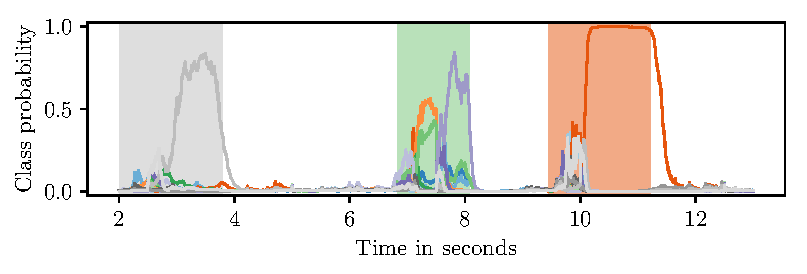
\includegraphics{figures/methods/framewise}
  \caption{Class probabilities attained from a framewise classifier. The shaded
    regions in the background designate the ground-truth.}
  \label{fig:framewise-p}
\end{figure}

Figure \ref{fig:framewise-p} illustrates the output of a framewise classifier.
Since the the \texttt{<blank>} class makes up about 50\% of the training data,
the classifier recognizes non-gesture data with high accuracy. When an activity
is detected, the classifier assigns high probabilities to multiple classes at
first until it discerns a single label as the correct one. This initial
confusion could most likely be alleviated with a backward pass in a
bidirectional RNN.

\section{Hidden Markov Model Decoding}
\label{sec:hmm}

A framewise classifier tells us which gesture most likely happened at each point
in time but a \texttt{swipe-down} gesture might be classified as
\texttt{rotate-outward} for the first few milliseconds, then \texttt{swipe-up}
for another few and finally as \texttt{swipe-down} for the rest of the activity.
This sequence of probability distributions now needs to be deciphered into just
a single \texttt{swipe-down} label. One way of doing just this is with hidden
Markov models (HMMs).

% TODO: graphical HMM model with states and emissions

% TODO: Markov property, Markov models, viterbi algorithm
A hidden Markov model consists of a Markov chain of hidden states $z^{(t)} \in
\{ 1, \dots, K \}$ and an observation model $x^{(t)}$. A Markov chain is a
probability distribution over sequences of arbitrary length where the transition
probability between states only depends on the current state, so
\begin{equation*}
  p\left( z^{(t)} | z^{(1)}, \dots, z^{(t - 1)} \right) = p\left( z^{(t)} | z^{(t - 1)} \right).
\end{equation*}
The transition model is usually written as a transition matrix $A$ where
$A_{ij}$ is the probability of transitioning from state $i$ into state $j$. The
initial probabilities for $z^{(1)}$ are given by a vector $\pi \in
\mathbb{R}^{K}$. The observation model specifies $p(x^{(t)} | z^{(t)})$ where
the observation probabilities only depend on the current state. In our case, the
observation model is categorical as well and specified by an observation matrix
$B$ where $B_{ij}$ gives the probability of observation $j$ in state $i$. 

A hidden Markov model models a situation where a state of interest is only
indirectly observable through emissions at each timestep. We have a sequence of
local classifications of each frame into of 17 classes and would like to derive
the true underlying sequence of gestures. An HMM lets us incorporate the
knowledge that a state $i$ might be observed as any other state for a short
while through the observation matrix $B$.

An efficient algorithm to decode an observation sequence into the most likely
underlying state sequence is \emph{Viterbi decoding}. It produces the most
likely sequence of hidden states
\begin{align*}
  z^{(1)}, \dots, z^{(n)} & = \argmax_{z^{(1)}, \dots, z^{(n)}} p(z^{(1)}, \dots, z^{(n)} | x^{(1)}, \dots, x^{(n)})\\
                          & = \argmax_{z^{(1)}, \dots, z^{(n)}} p(z^{(1)}) \cdot \prod_{t = 2}^{n} p(z^{(t)} | z^{(t - 1)}) \cdot \prod_{t = 1}^{n} p(x^{(t)} | z^{(t)})\\
                          & = \argmax_{z^{(1)}, \dots, z^{(n)}} \log \pi_{z^{(1)}} + \sum_{t = 2}^{n} \log A_{z^{(t - 1)}, z^{(t)}} + \sum_{t = 1}^{n} \log p(x^{(t)} | z^{(t)})\\
  \intertext{given a sequence of observations. A problem is that a framewise classifier
produces $p(z^{(t)} | x^{(t)})$ instead of $p(x^{(t)} | z^{(t)})$. We can
rewrite the decoding objective with Bayes's theorem.}
                          & = \argmax_{z^{(1)}, \dots, z^{(n)}} \log \pi_{z^{(1)}} + \sum_{t = 2}^{n} \log A_{z^{(t - 1)}, z^{(t)}} + \sum_{t = 1}^{n} \left( \log p(z^{(t} | x^{(t)}) + \log p(x^{(t)}) - \log p(z^{(t)}) \right)\\
  \intertext{The $p(x^{(t)})$ term is irrelevant to the arg max because it does not depend on $z$.}
                          & = \argmax_{z^{(1)}, \dots, z^{(n)}} \log \pi_{z^{(1)}} + \sum_{t = 2}^{n} \log A_{z^{(t - 1)}, z^{(t)}} + \sum_{t = 1}^{n} \left( \log p(z^{(t} | x^{(t)}) - \log p(z^{(t)}) \right)\\
                          & = \argmax_{z^{(1)}, \dots, z^{(n)}} \log \pi_{z^{(1)}} + \sum_{t = 2}^{n} \log A_{z^{(t - 1)}, z^{(t)}} + \sum_{t = 1}^{n} \log p(z^{(t} | x^{(t)})
\end{align*}
The last line is true if $\pi$ is the stationary distribution of the Markov
chain $A$, i.e. the long term distribution over hidden states, because then
$p(z^{(1)}) = \pi$ and $p(z^{(t)}) = Ap(z^{(t - 1)}) = \pi$. Therefore $\log
p(z^{(t)})$ is actually independent of $z^{(t)}$ and can be ignored.

The Viterbi algorithm finds the maximizer by computing the probability of being
in state $j$ at time $t$ given that you take the most probable path.
\begin{equation*}
  \delta_{t}(j) = \max_{z^{(1)}, \dots, z^{(t - 1)}} p(z^{(1)}, \dots, z^{(t - 1)}, z^{(t)} = j | x^{(1)}, \dots, x^{(t)})
\end{equation*}
The key insight here is that the most probable path to state $j$ at time $t$
must be the one that maximizes the joint probability of being in state $k$ at
time $t - 1$ and transitioning from $k$ to $j$, i.e.
\begin{equation*}
  \delta_{t}(j) = \max_{i} \delta_{t - 1}(i) \cdot A_{ij} \cdot B_{j,x^{(t)}}
\end{equation*}
If you compute $\delta$ for $t$ from 1 to $n$ and store the maximizer $i$ in
another table $\alpha_{tj}$, you can find the most probable final state as
$z^{(n)} = \argmax_{i} \delta_{n}(i)$ and work your way back to $t = 1$ by
following the $\alpha_{n,z^{(n)}}$ to the predecessor state and so forth.
This explanation is summarized from \cite{murphy12}.

Since we do not work with the observation matrix $B$, the process of
constructing an HMM decoder from the training data is reduced to finding $A$ and
$\pi$. The structure of $A$ allows us to include our domain knowledge in the
decoding process. We want to encode in $A$ that no two gestures transition
directly from one to another, there is always a \texttt{<blank>} in between, and
the probability of staying in the same state is high because a gesture is at
least a thousand frames long. So we define the $A_{i,17}$ entries, the
transition probability from gesture $i$ to \texttt{<blank>}, as the proportion
of frames belonging to class $i$ that transition to \texttt{<blank>} and
$A_{i,i}$, the self-transition probability, as $1 - A{i,17}$. The transition
probability from \texttt{<blank>} to any of the gestures is the proportion of
gesture frames following blank frames and its self-transition probability is the
complement of that. Finally, we choose $\pi$ as the stationary distribution of
$A$.

\begin{figure}
  \centering
  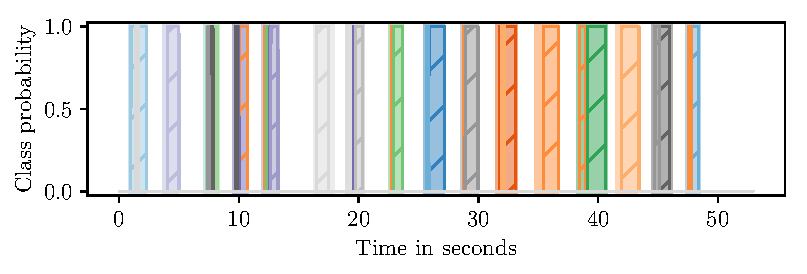
\includegraphics{figures/methods/decoded}
  \caption{A decoding produced by an HMM decoder. The shaded regions in the
    background denote the ground-truth.}
  \label{fig:decoded}
\end{figure}

\section{Hidden Markov Model Segmentation}
\label{sec:hmm-segmentation}

Figure \ref{fig:decoded} shows that an HMM decoder is able to recognize the
points of activity in a sequence of local classifications and is also reasonably
accurate in decoding them into the correct class. However, there are a lot of
spurious labels mixed in with the correct labels. The idea of HMM segmentation
is to divide the decoding process into two parts. First, an HMM with just two
states, \texttt{<gesture>} and \texttt{<blank>}, segments the sequence and
afterwards a second HMM produces a single label for each segment. The result of
this is depicted in Figure \ref{fig:segmented}.

\begin{figure}
  \centering
  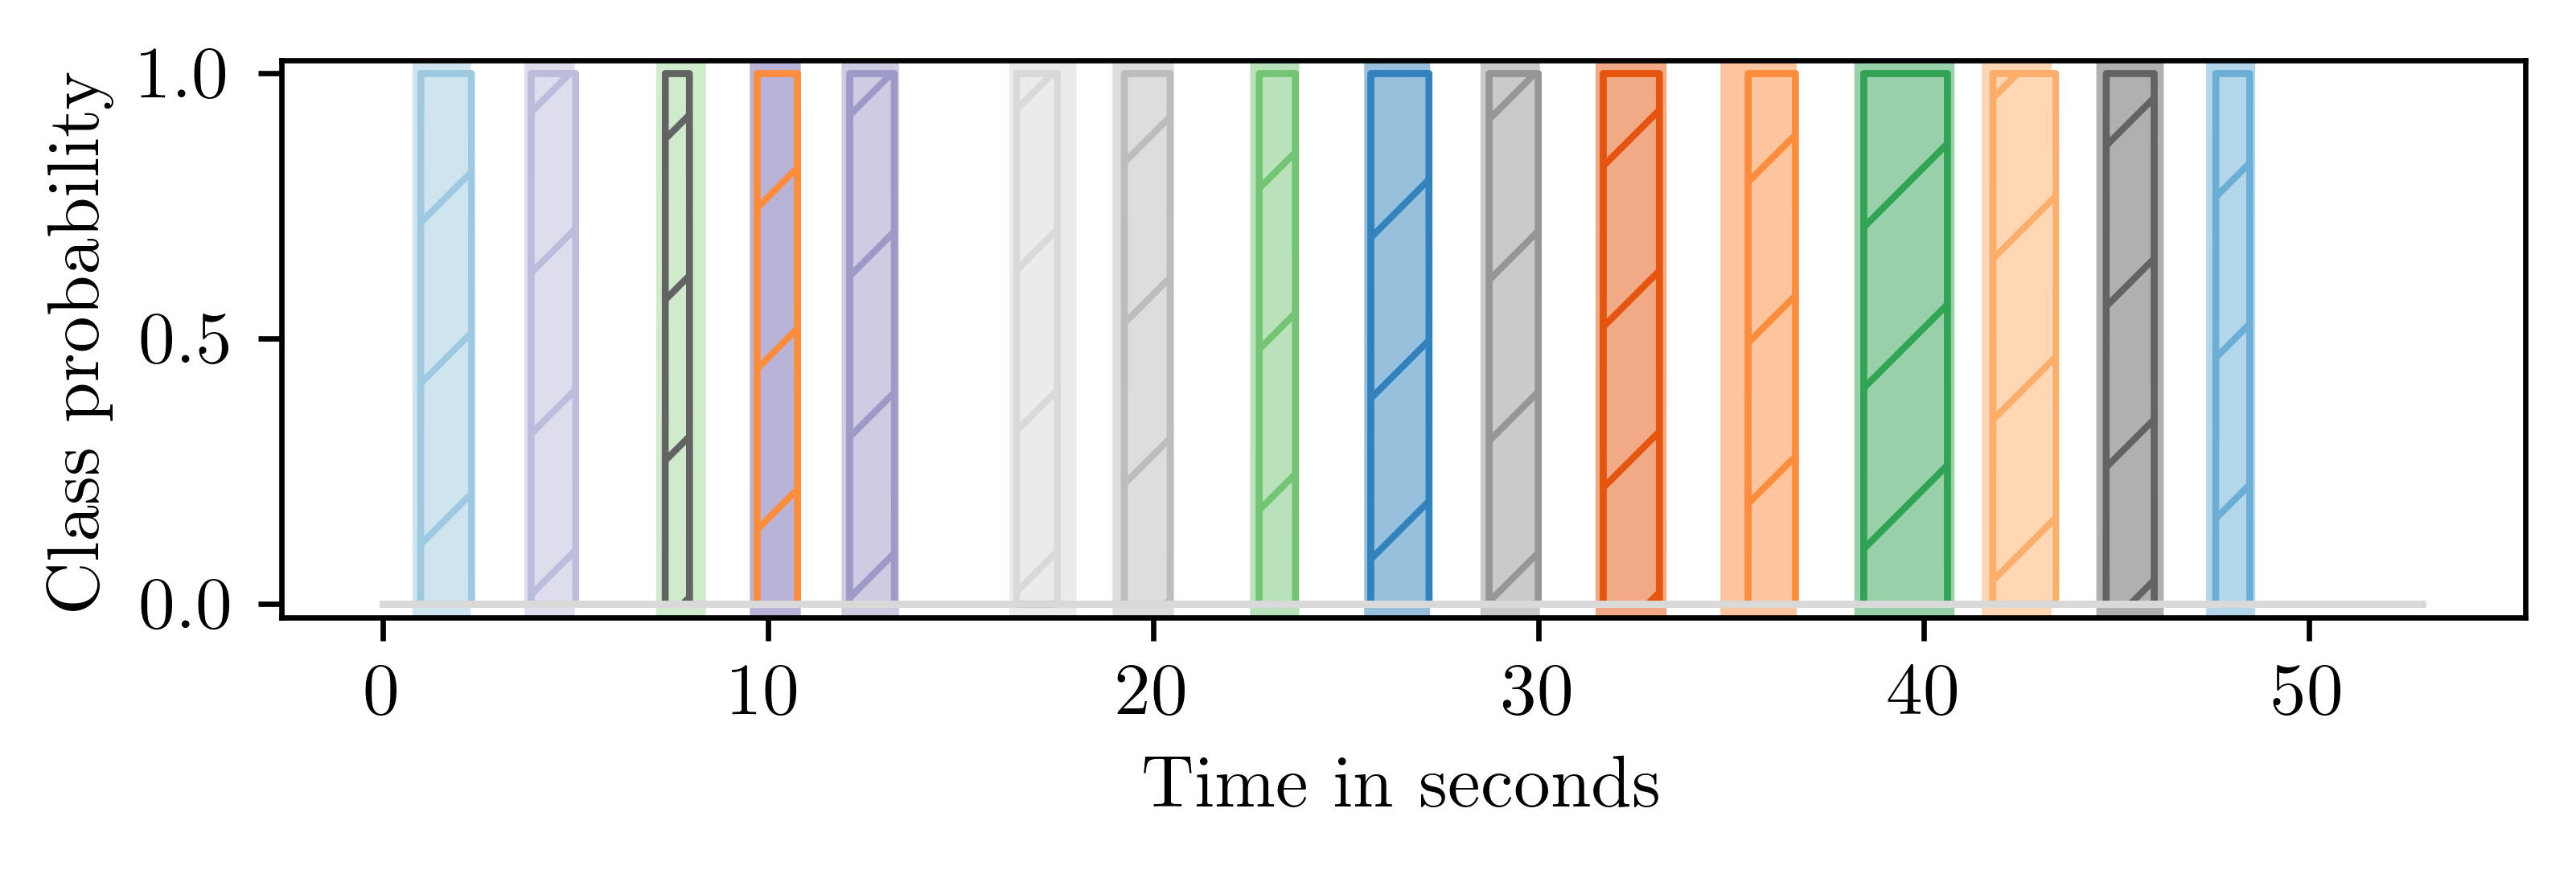
\includegraphics{figures/methods/segmented}
  \caption{A decoding produced by an HMM segmenter followed by segment decoding}
  \label{fig:segmented}
\end{figure}

The HMM segmenter is constructed in the same way as the decoder in Section
\ref{sec:hmm} with the twist that all gestures are combined into a single hidden
state \texttt{<gesture>}. When the HMM segments a recording, the probability of
the \texttt{<gesture>} state is the sum of all gesture probabilities. To suppress
the remaining spurious activations, we also filter out all segments that are
shorther than \SI{500}{\milli\second} because we know from the dataset
statistics that the shortest gesture is over a second long on average. Therefore
anything shorther than half of that is most certainly erroneous.

The decoding HMM is particularly simple in that the initial distribution $\pi$
is the uniform distribution and the transition matrix $A$ is the identity matrix
thus disallowing any transitions. After viterbi decoding, the segment label is
$z^{(n)}$.

\section{Connectionist Temporal Classification}
\label{sec:ctc}

\begin{figure}[h]
  \centering
  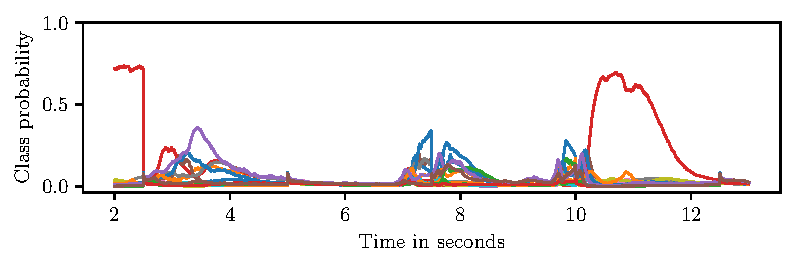
\includegraphics{figures/methods/ctc}
  \caption{Class probabilities attained with CTC}
  \label{fig:ctc-p}
\end{figure}

In the combined approach with neural network and HMM, we train two different
systems in series and the NN.

Training with categorical cross entropy tries to categorize short windows of events correctly.
However, this is not actually what we want and may also be impossible to do.
For example, the gestures extend-index-finger and tap-index-finger start the exact same way, so the first few events are not distinguishable.
With CTC we might be able to get the network to stay quiet until it is sure, which type of gesture it is, instead of forcing it to predict one of them at inappropriate times.

% TODO: Training problems because of long sequences and the need to store all
% intermediate results for BPTT. Sequences without any labels cannot be handled.

% TODO: Chunk size is 250 but RNNs can still learn longer sequences empirically,
% see Graves handwriting paper.
